\documentclass[onecolumn, draftclsnofoot,10pt, compsoc]{IEEEtran}
\usepackage{url}
\usepackage{tabu}
\usepackage{color}    % colors for code listings
\usepackage{float}
\usepackage{caption}
\usepackage{geometry}
\usepackage{graphicx}
\usepackage{listings} % code listings
\usepackage{pdfpages} % for inserting pdfs into LateX
\usepackage{pgfgantt}
\usepackage{setspace}

\graphicspath{{images/}}
\geometry{textheight=9.5in, textwidth=7in, margin=0.75in}

%%%%%%%%%%%%%%%%%%%%%%%%%%%%%%%%%%%%%%%%%%%%%%%%%%%%%%%%%%%%%%%%%%%%%%%%%%%%%%%%%%%%%%%%%%%%%%%%%%%
% Code listing options %
\definecolor{mygreen}{rgb}{0,0.6,0}
\definecolor{mygray}{rgb}{0.5,0.5,0.5}
\definecolor{mymauve}{rgb}{0.58,0,0.82}

\lstset{ 
  backgroundcolor=\color{white},   % choose the background color
  basicstyle=\footnotesize,        % size of fonts used for the code
  breaklines=true,                 % automatic line breaking only at whitespace
  captionpos=b,                    % sets the caption-position to bottom
  commentstyle=\color{mygreen},    % comment style
  escapeinside={\%*}{*)},          % if you want to add LaTeX within your code
  keywordstyle=\color{blue},       % keyword style
  stringstyle=\color{mymauve},     % string literal style
}
\lstdefinestyle{customc}{
  belowcaptionskip=1\baselineskip,
  breaklines=true,
  frame=L,
  xleftmargin=\parindent,
  language=C,
  showstringspaces=false,
  basicstyle=\footnotesize\ttfamily,
  keywordstyle=\bfseries\color{mygreen},
  commentstyle=\itshape\color{mygreen},
  identifierstyle=\color{blue},
  stringstyle=\color{orange},
}
%%%%%%%%%%%%%%%%%%%%%%%%%%%%%%%%%%%%%%%%%%%%%%%%%%%%%%%%%%%%%%%%%%%%%%%%%%%%%%%%%%%%%%%%%%%%%%%%%%%
% 1. Fill in these details
\def \CapstoneTeamName{     TeamName}
\def \CapstoneTeamNumber{       24}
\def \GroupMemberOne{            Ciin S. Dim}
\def \GroupMemberTwo{           Louis Leon}
\def \CapstoneProjectName{      Kinect Based Virtual Therapy Solution}
\def \CapstoneSponsorCompany{   OSU Healthcare Systems Engineering Lab}
\def \CapstoneSponsorPerson{        Mehmet Serdar Kilinc}

% 2. Uncomment the appropriate line below so that the document type works
\def \DocType{      %Problem Statement
                %Requirements Document
                %Technology Review
                %Design Document
                Final Report
                }
            
\newcommand{\NameSigPair}[1]{\par
\makebox[2.75in][r]{#1} \hfil   \makebox[3.25in]{\makebox[2.25in]{\hrulefill} \hfill        \makebox[.75in]{\hrulefill}}
\par\vspace{-12pt} \textit{\tiny\noindent
\makebox[2.75in]{} \hfil        \makebox[3.25in]{\makebox[2.25in][r]{Signature} \hfill  \makebox[.75in][r]{Date}}}}
% 3. If the document is not to be signed, uncomment the RENEWcommand below
\renewcommand{\NameSigPair}[1]{#1}

%%%%%%%%%%%%%%%%%%%%%%%%%%%%%%%%%%%%%%%%%%%%%%%%%%%%%%%%%%%%%%%%%%%%%%%%%%%%%%%%%%%%%%%%%%%%%%%%%%%
\begin{document}
\begin{titlepage}
    \pagenumbering{gobble}
    \begin{singlespace}
        %\includegraphics[height=4cm]{coe_v_spot1}
        \hfill 
        % 4. If you have a logo, use this includegraphics command to put it on the coversheet.
        %\includegraphics[height=4cm]{CompanyLogo}   
        \par\vspace{.2in}
        \centering
        \scshape{
            \huge CS Capstone\DocType \par
            {\large Spring Term}\par
            {\large\today}\par
            \vspace{.5in}
            \textbf{\Huge\CapstoneProjectName}\par
            \vfill
            {\large Prepared for}\par
            \Huge \CapstoneSponsorCompany\par
            \vspace{5pt}
            {\Large\NameSigPair{\CapstoneSponsorPerson}\par}
            {\large Prepared by }\par
            Group\CapstoneTeamNumber\par
            % 5. comment out the line below this one if you do not wish to name your team
            %\CapstoneTeamName\par 
            \vspace{5pt}
            {\Large
                \NameSigPair{\GroupMemberOne}\par
                \NameSigPair{\GroupMemberTwo}\par
            }
            \vspace{20pt}
        }
        \begin{abstract}
        % 6. Fill in your abstract    
        The purpose of this document is to summarize the progress made towards this project over the first half of Spring Term. The document includes the project purpose, goals, current project state, problems impeding progress and solutions, and remaining tasks.
    \end{abstract}     
    \end{singlespace}
\end{titlepage}
\newpage
\pagenumbering{arabic}
\tableofcontents
% 7. uncomment this (if applicable). Consider adding a page break.
\listoffigures
%\listoftables
\clearpage

% 8. now you write!
\section{Purpose}
The purpose of the Kinect Based Physical Therapy Solution project is to provide a solution for physical therapy patients diagnosed with Parkinson's disease to perform in-home therapy exercises. This solution will not only allow for an interactive way of completing a patient's required home therapy but will provide a way for their physical therapist to track their progress and monitor their exercises.

\section{Goals}
Our project will have a simple UI that can be easily navigated by a user with Parkinson's Disease. From the UI, the user will be able to select the option that allows them to select and do the available exercises. Our goal is to have two different exercises available to the user to choose from. One of our stretch goals is to be able to have a physical therapist prescribe exercises and specify frequency. The program will guide the user through these exercises using text and verbal instructions. One of our stretch goals is to implement visual (graphical) cues (over-laying their body on the camera feed) to the user to guide them through exercises. As the user performs exercises, their node data will be collected to be sent to their physical therapist as a .csv file, and it will be used for report generation. We will define the exercise's correct movements and compare them to the user's node data. This is how we will analyze the data to determine user accuracy for report generation. Another option the user will be able to select is report generation. This will display the user's performance data in graphs and charts, showing their progress with the exercises over time. 

\section{Project Introduction}
\subsection{Project Information}
The Kinect Based Physical Therapy project was requested by the OSU Healthcare Systems Engineering Lab, specifically by our client Dr. Mehmet Serdar Kilinc. The Healthcare System Engineering Lab in OSU is a research center which focuses on innovative non-traditional healthcare models, information technology healthcare interventions, and translational research. The lab is currently focusing on research projects that require sensor-based healthcare solutions. This project was specifically focused on using a Microsoft Kinect Sensor with the assumption being it could be useful for in-home health monitoring applications.

The importance of this project was to demonstrate a proof of concept that helps people with neurodegenerative conditions such as Parkinson's Disease get access to physical therapy remotely without the need for in-person therapy sessions. Access to physical therapy clinics is problematic due to physical disability that inhibits traveling and can be costly for patients. Non-wearable sensor-based solutions have the potential to reduce the number of in-person visits and the long-distance traveling that is required. 

\subsection{Team Members}
The two members of the development team for this project were Louis Leon and San Dim Ciin, two senior Computer Science students at Oregon State University. They both held the role as lead developers for this project. Each team member had large tasks in all the components of the project which ranged from building the user interface to automating the report generation process. The project's client, Dr. Kilinc supervised the project's direction and progress. He provided feedback at various stages of the development process and requested features that could serve as additions to the project overall. 

\section{Requirements}
*Insert Requirements Document Here*

\includepdf[pages=-, pagecommand={}]{requiredDocuments/Requirements}  
\subsection{Requirement Changes}
*Add (your client should have okay'd): What new requirements were added? What existing requirements were changed? What existing requirements were deleted? Why?* 
\subsection{Final Project Timeline}
*Add: Final Gantt Chart as a record of what happened when.* 


\section{Design}
*Insert Design Document Here*

\includepdf[pages=-, pagecommand={}]{requiredDocuments/DesignDocument}  
\cite{KinectDevelop}
\subsection{Design Changes}
*Add (your client should have okay'd): What design aspects were changed, deleted or added? Why?*


\section{Technology Review}
*Insert Tech Review Document Here*

\section{Team Blog}

\section{Final Poster}
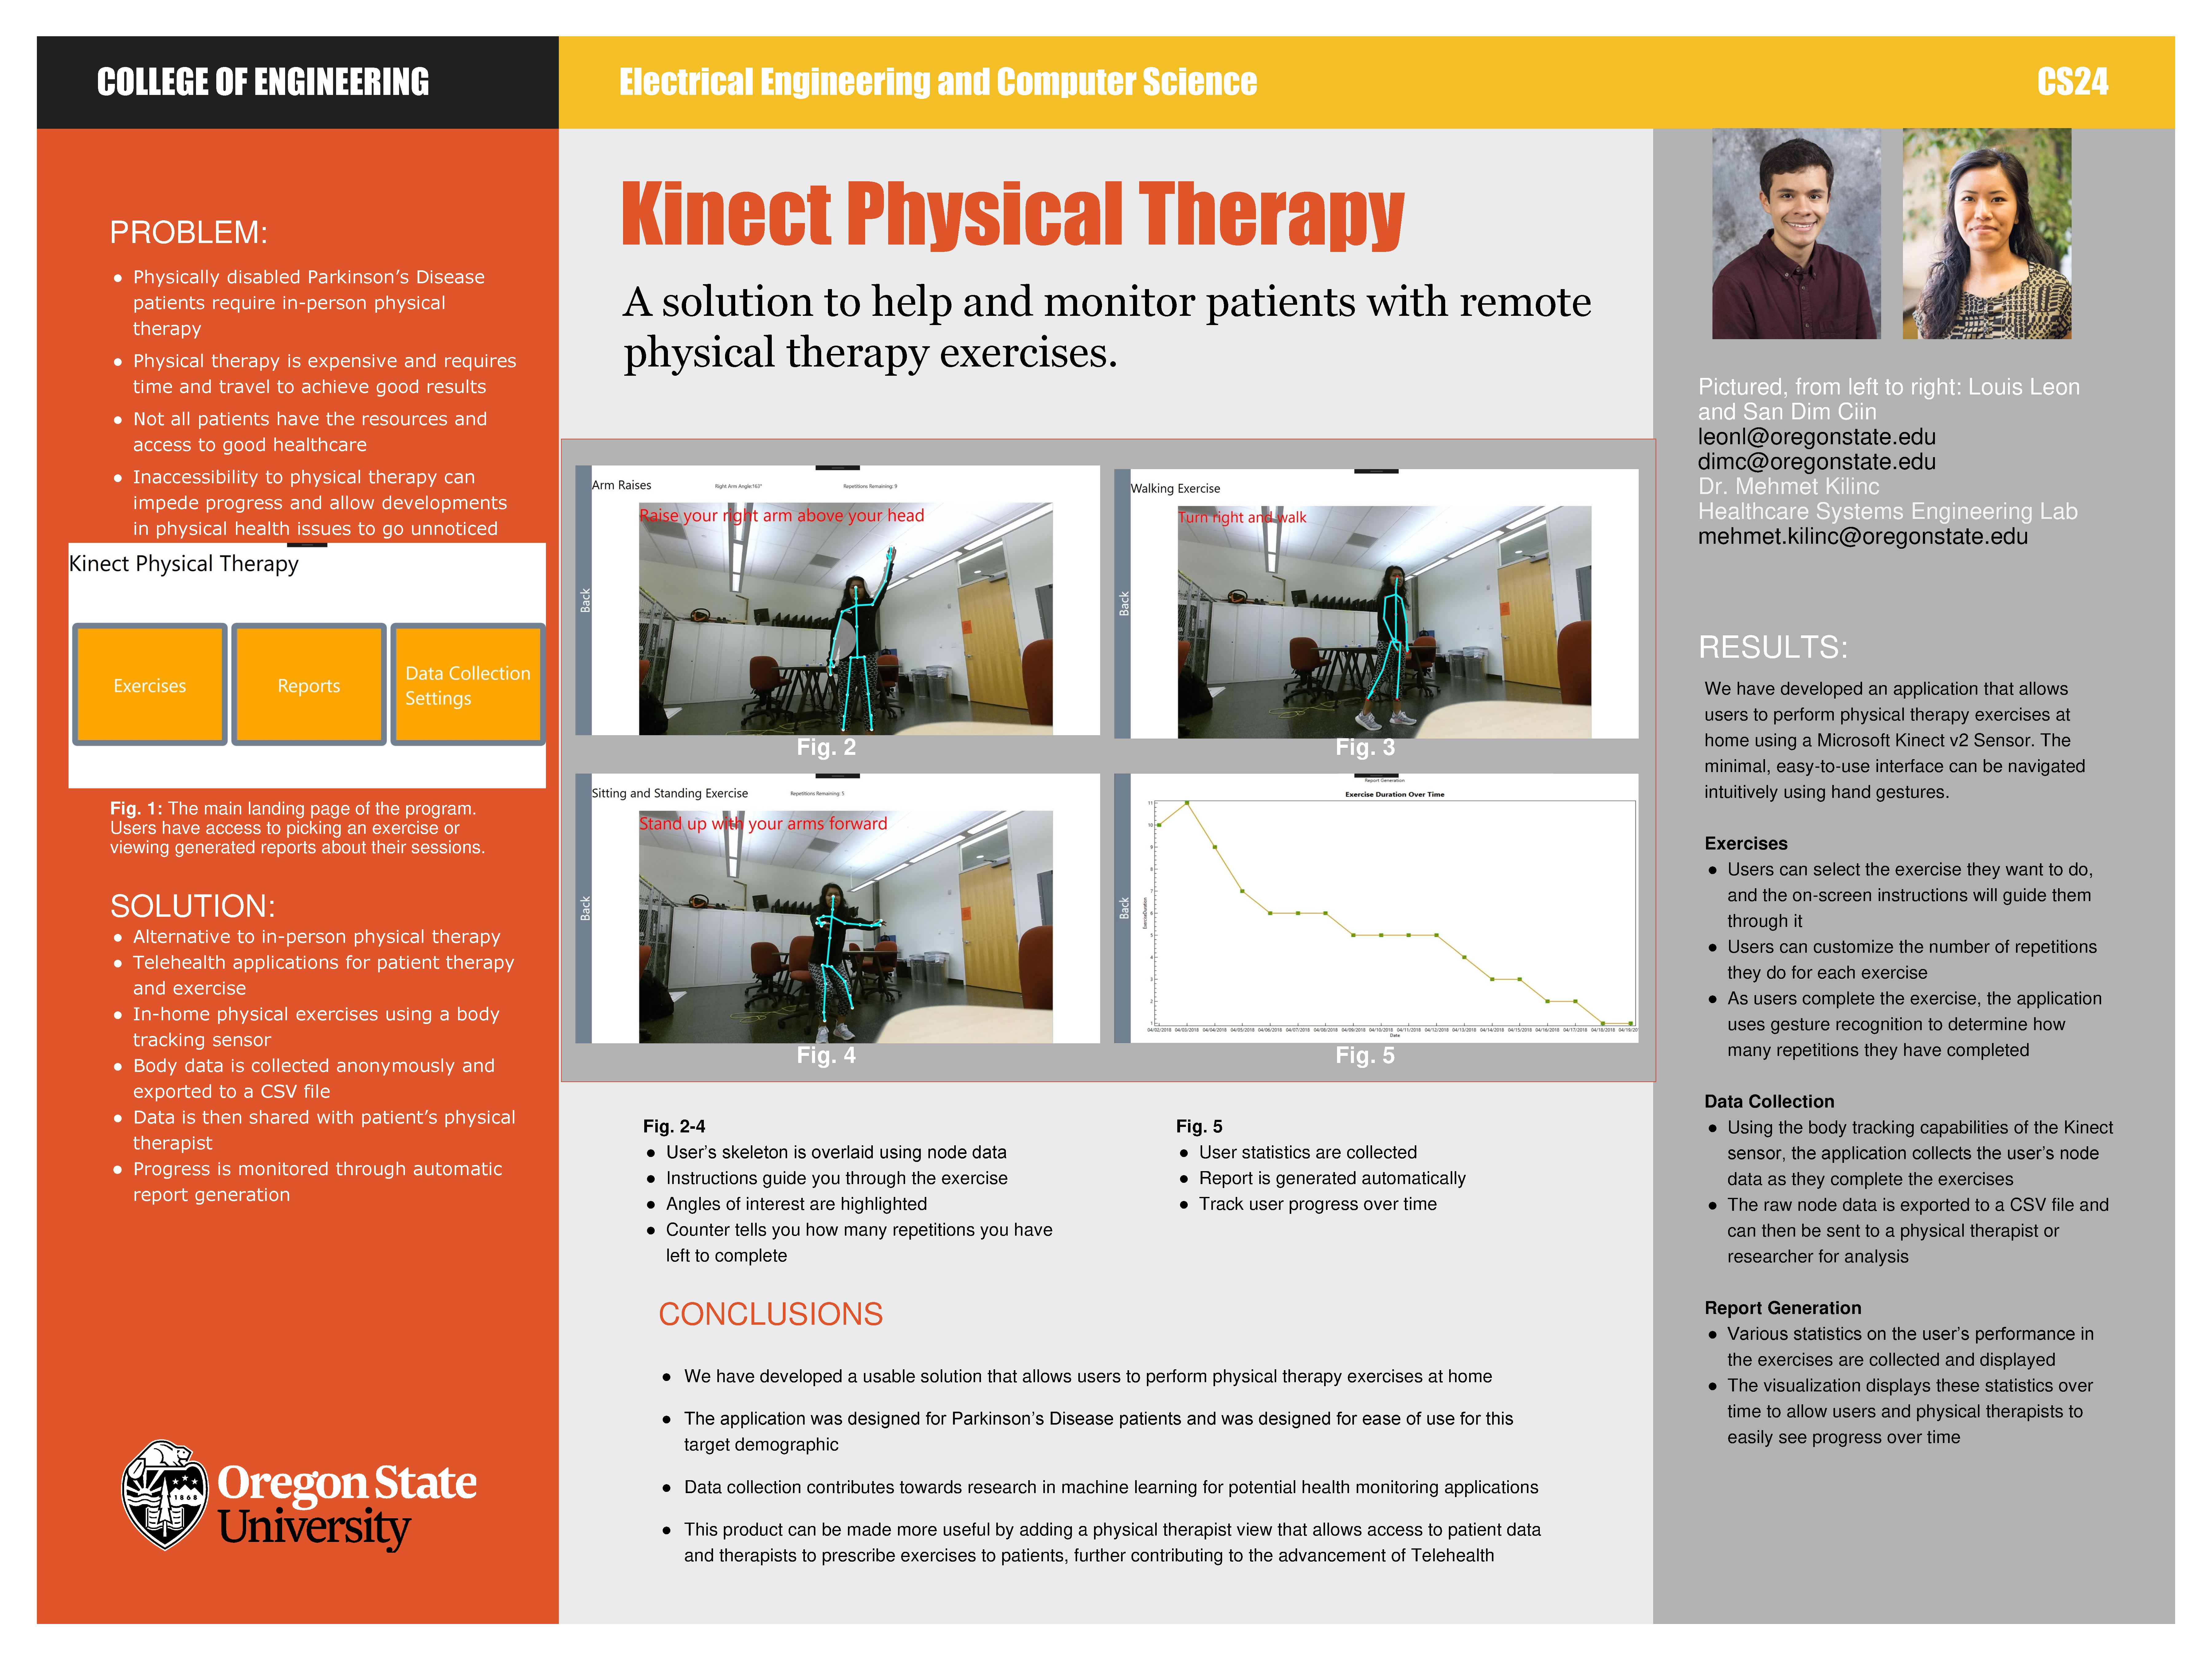
\includepdf[pages=-, pagecommand={},landscape=true]{requiredDocuments/FinalPoster}  
\section{Project Documentation}
\subsection{Installation and Building}

\subsection{System Requirements}

\subsection{User Guide}

\section{Recommended Technical Resources}
\subsection{Useful Websites}

\section{Conclusions and Reflections}
\begin{flushleft}
{\large\textbf{Louis Leon}\par}
\textbf{What technical information did you learn?}\par

\textbf{What non-technical information did you learn?}\par

\textbf{What have you learned about project work?}\par

\textbf{What have you learned about project management?}\par

\textbf{What have you learned about working in teams?}\par

\textbf{If you could do it all over, what would you do differently?}\par

\end{flushleft}

\begin{flushleft}
{\large\textbf{San Dim}\par}
\textbf{What technical information did you learn?}\par

\textbf{What non-technical information did you learn?}\par

\textbf{What have you learned about project work?}\par

\textbf{What have you learned about project management?}\par

\textbf{What have you learned about working in teams?}\par

\textbf{If you could do it all over, what would you do differently?}\par

\end{flushleft}

\section{Appendix I: Essential Code Listings}
\begin{figure}[H]
\begin{lstlisting}[language=C, style=customc]
 public PlotModel OpenTimes(string file)
        {
            var doc = new CsvDocument();
            doc.Load(file);
            var tmp = new PlotModel { Title = "Exercise Duration Over Time" };
            tmp.IsLegendVisible = false;
            tmp.PlotMargins = new OxyThickness(50, 0, 0, 40);
            for (int i = 1; i < doc.Headers.Length; i++)
            {
                var ls = new ScatterSeries { Title = doc.Headers[i] };
                foreach (var item in doc.Items)
                {
                    var t1 = DateTime.Parse(item[0]);
                    var t2 = DateTime.Parse(item[i]);
                    double x = DateTimeAxis.ToDouble(t2);
                    double y = DateTimeAxis.ToDouble(t1.Minute);
                    ls.Points.Add(new ScatterPoint(x, y));
                }
                tmp.Series.Add(ls);
            }
            for (int i = 1; i < doc.Headers.Length; i++)
            {
                var ls = new LineSeries { Title = doc.Headers[i] };
                foreach (var item in doc.Items)
                {
                    var t1 = DateTime.Parse(item[0]);
                    var t2 = DateTime.Parse(item[i]);
                    double x = DateTimeAxis.ToDouble(t2);
                    double y = DateTimeAxis.ToDouble(t1.Minute);
                    ls.Points.Add(new DataPoint(x, y));
                }
                tmp.Series.Add(ls);
            }
            tmp.Axes.Add(new LinearAxis
            {
                Position = AxisPosition.Left,
                Title = doc.Headers[0],
                TickStyle = TickStyle.Inside,
            });
            tmp.Axes.Add(new DateTimeAxis
            {
                Position = AxisPosition.Bottom,
                Title = doc.Headers[1],
                TickStyle = TickStyle.Inside,
                StringFormat = "MM/dd/yyyy"
            });
            return tmp;
        }
\end{lstlisting}
\caption{Report Generation with OxyPlot}
\end{figure}

\section{Appendix II: Related Project Information}


\bibliographystyle{ieeetr}
\bibliography{FinalReport}
\end{document}
